\documentclass[12pt,letterpaper]{article}
%sets the paper's header
\newcommand{\sethead}[6]{
	\lhead{\textit{#1}}
	\rhead{#2\\#3\\#4\\#5\\#6}
}
\usepackage[utf8]{inputenc}
%headings
\usepackage{fancyhdr}
%double-space
\usepackage{setspace}
%variable margins
\usepackage{geometry}
%make the margins a bit less ridiculous
\newgeometry{top=1in,bottom=1.5in,left=1in,right=1in}
%images
\usepackage{graphicx}
\usepackage{amsmath}
\usepackage{amsfonts}
\usepackage{graphicx}
\pagestyle{fancy}

\begin{document}
	%ragged right with paragraph indents
    \newlength{\saveparindent}
	\setlength{\saveparindent}{\parindent}
	\raggedright
	\setlength{\parindent}{\saveparindent}
    
    %%%%%%%%%%%%%%%%%%%%%%%%%%%%%%%%%%%%%%%%%%%%%%%%%%%%
	%%     I   M   P   O   R   T   A   N   T   :      %%
    %%  please remember to set the header to reflect  %%
    %%      the class that you're writing for!        %%
    %%%%%%%%%%%%%%%%%%%%%%%%%%%%%%%%%%%%%%%%%%%%%%%%%%%%
	\sethead{Homework 2}{Joshua Kuroda}{Jenny Miller}{CMSI 282}{Toal}{03/03/15}
    
	%spacing
	\doublespacing
    \begin{center}
		%necessary spacing between the header and the body
	\end{center}
    
    %Paper goes here!
    \begin{enumerate}
    \item
      \begin{enumerate}
      \item f = \(\Theta\)(g)
      \item f = \(\Omega\)(g)
      \item f = \(\Omega\)(g)
      \item f = \(\Omega\)(g)
      \item f = \(\Omega\)(g)
      \item f = \(\Omega\)(g)
      \item f = \(O\)(g)
      \item f = \(\Omega\)(g)
      \item f = \(\Omega\)(g)
      \item f = \(O\)(g)
      \item f = \(\Omega\)(g)
      \item f = \(\Omega\)(g)
      \item f = \(\Omega\)(g)
      \item f = \(\Theta\)(g)
      \item f = \(O\)(g)
      \item f = \(\Omega\)(g)
      \item f = \(\Omega\)(g)
      \end{enumerate}
    \item
      \begin{enumerate}
      \item
        $
        \begin{array}{cc}
        a & b \\
        c & d \\
        \end{array}$
        •
        $
        \begin{array}{cc}
        e & f \\
        g & h \\
        \end{array}$
        =
        $
        \begin{array}{cc}
        ae + bg & af + bh \\
        ce + dg & cf + dh \\
        \end{array}$
      \item
        Let's think about the example of $X^8$. If we separate each X and then 			square them over and over, we can show how many matrix multiplications 			are necessary.
        \newline
        $X^8$ = X $\ast$ X $\ast$ X $\ast$ X $\ast$ X $\ast$ X $\ast$ X $\ast$ X
        \newline
        So we only need to multiply X $\ast$ X one time to get $X^2$. This means 		 that we can replace the other three sets of multiplication with that 			answer, getting:
        \newline
        $X^8$ = $X^2$ $\ast$ $X^2$ $\ast$ $X^2$ $\ast$ $X^2$
        \newline
        Now we can see that it is only necessary to multiply $X^2$ $\ast$ $X^2$ 		once to get $X^4$. So now we can replace the second multiplication with 		that answer, getting:
        \newline
        $X^8$ = $X^4$ $\ast$ $X^4$
        \newline
        Finally, our third multiplication brings us to 3 = $log_2$(8). So 				extending this finding to $X^n$, we see that the number of arithmetic 			operations needed is \(O\)(log(n)). $\Box$
      \end{enumerate}
    \item
      By definition, the length of any binary integer \(x\) is 				 		  floor($log_2$(\(x\))) + 1 and the length of any decimal integer \(y\) 		  is ceil($log_2$(\(y\))). Let's start by simplifying the following:
      \begin{center}
      floor($log_2$(\(x\))) + 1 \(\leq\) 4 $\ast$ ceil($log_{10}$(\(x\)))
      \end{center}
      Because of the $floor$ function, we know that:
      \begin{center}
      floor($log_2$(\(x\))) + 1 $<$ $log_2$(\(x\)) + 1
      \end{center}
      Further,
      \begin{center}
      $log_2$(\(x\)) $<$ $log_2$(\(x\)) + 1
      \end{center}
      Due to the $ceil$ function,
      \begin{center}
      4 $\ast$ ceil($log_{10}$(\(x\))) $>$ 4 $\ast$ $log_{10}$(\(x\))
      \end{center}
      Thus, we have:
      \begin{center}
      $log_2$(\(x\)) \(\leq\) 4 $\ast$ $log_{10}$(\(x\))
      \end{center}
      Changing bases, we get:
      \begin{center}
  	  $log_{10}$(\(x\)) = $log_2$(\(x\)) / $log_2$(10)
      \end{center}
      Therefore,
      \begin{center}
      $log_2$(\(x\)) $\ast$ $log_2$(10) $\leq$ 4
      \end{center}
      So any binary integer $x$ is at most four times as long as the 			 	   corresponding decimal integer. $\Box$
    \item
      Call $f_1$ = $log$($n!$) and $f_2$ = $n$ $log$($n$). We are going to show 	  that both functions are bounded from above by $log$($n^n$) and bounded 		  from below by $log$($(n/2)^{(n/2)}$).
      The graph below shows $f_1$ vs. $log$($n^n$). The line that is 	      		  bounding $f_1$ from above is $log$($n^n$).
      \begin{center}
      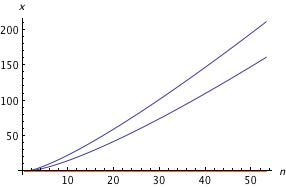
\includegraphics{Graph3.jpg}
      \end{center}
      This illustration shows us that $log$($n^n$) is the upper bound on 			  $log$($n!$).
      In the next graph we have $log$($n!$) vs. $log$($(n/2)^{(n/2)}$). The line 	   that is bounding $f_1$ from below is $log$($(n/2)^{(n/2)}$).
      \begin{center}
      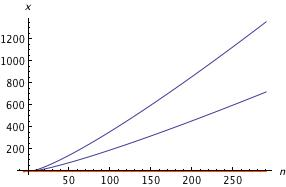
\includegraphics{Graph2.jpg}
      \end{center}
      Now let's compare using $f_2$ instead of $f_1$. The graph below shows $n$ 	  $log$($n$) vs. $log$($n^n$). There looks to be only one line because both 	  functions describe the same graph by definition of log identities.
      \begin{center}
      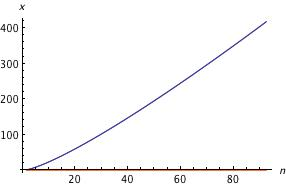
\includegraphics{Graph4.jpg}
      \end{center}
      This illustration shows us that $log$($n^n$) bounds $n$ $log$($n$) from  		  above.
      In the next graph we have $n$ $log$($n$) vs. $log$($(n/2)^{(n/2)}$). The 		  line that bounds $f_2$ from below is $log$($(n/2)^{(n/2)}$).
      \begin{center}
      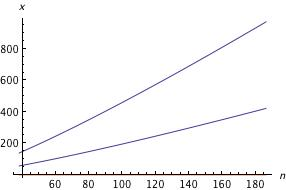
\includegraphics{Graph5.jpg}
      \end{center}
      We have compared $f_1$ and $f_2$ to both $log$($n^n$) and 					  $log$($(n/2)^{(n/2)}$) and found that both $f_1$ and $f_2$ are bounded from 		above by $log$($n^n$). Further, both $f_1$ and $f_2$ are bounded from below 	  by $log$($(n/2)^{(n/2)}$). We have fully bounded both functions, thus 		  $log$($n!$) = \(\Theta\)($n$ $log$($n$)). $\Box$
    \item
      $4^{1536}$ (mod 35) = 1
      \newline
      $9^{4825}$ (mod 35)	= 1
      \newline
      1 - 1 (mod 35) = 0
      \newline
      Thus, $4^{1536}$ - $9^{4825}$ is divisible by 35.
    \item
      Using Fermat's Little Theorem, we know that 31 is prime.
      \newline
      $5^{30}$ = 1 (mod 31)
      \newline
      $6^{30}$ = 1 (mod 31)
      \newline
      Now, $5^{30000}$ = $5^{rem(30000, 30)(mod 31))}$ = 1
      \newline
      $6^{123456}$ = $6^6$ $\ast$ $6^{123450}$ = $6^6$ $\ast$ $6^{rem(123450,30) 	   (mod 31)}$ = $6^6$ (mod 31) = 1
      \newline
      $5^{30000}$ - $6^{123456}$ = (1 - 1)(mod 31) = 0
      \newline
      Thus, the difference of $5^{30000}$ and $6^{123456}$ is a multiple of 31.
    \item
      For $b$ = 15, the repeated squaring method uses 6 multiplications, as shown 		below:
      \newline
      $a^{15}$ = $x$ $\ast$ ($x$ $\ast$ [$x$ \(\ast\) \(x^2\)]$^2$\()^2\)
      \newline
      However, using addition-chain exponentiation, only 5 multiplications are 	   	   needed if $x^3$ is re-used, as shown below:
      \newline
      $a^{15}$ = $x^3$ $\ast$ ([$x^3$\(]^2\)$)^2$
    \item
      $2^{125}$ (mod 127) = 64
    \item
      $problem9.rb$
      \newline
      The running time of this algorithm is \(O\)(n).
    \item
      Wilson's theorem cannot be used as the basis for a primality test because 	  of the fact that it is ineffective as a test in practice. This is because 	  computing ($N$ - 1)! mod $N$ for large $N$ is difficult, and other 			  primality tests can be used that would be faster and more efficient.
    \item
      $problem11.py$
    \end{enumerate}
    
\end{document}